%%==============================================================================
%% Beamer template for IFPEN slides
%%==============================================================================

\documentclass[aspectratio=169]{beamer}

\usetheme{Madrid}
\usepackage[utf8]{inputenc}
\usepackage[T1]{fontenc}
\usepackage{times}
\usepackage{xcolor}
\usepackage{listings}
\usepackage{tabto}
\usepackage{multimedia}
\usepackage{animate}
\usepackage{ragged2e}
\usepackage{tikz}
\usepackage{multimedia}
\usepackage{wallpaper}
%\usepackage{siunitx}
\usepackage{bm}
% \usepackage[english]{babel}
\usepackage{natbib}
% \bibliographystyle{unsrtnat}
\bibliographystyle{apalike}
\usetikzlibrary{positioning}

\lstdefinestyle{globallistingstyle}{basicstyle=\tiny\ttfamily,frame=single,showstringspaces=false}
\lstdefinestyle{bash}{language=bash,
                      basicstyle=\small\ttfamily,
                      commentstyle=\color{green},
                      keywordstyle=\color{blue},
                      stringstyle=\color{red},
                      backgroundcolor=\color{lightpurple}}
\lstdefinestyle{tinybash}{language=bash,
                      basicstyle=\tiny\ttfamily,
                      commentstyle=\color{green},
                      keywordstyle=\color{blue},
                      stringstyle=\color{red},
                      backgroundcolor=\color{lightpurple}}
\lstdefinestyle{C++}{language=C++,
                     style=globallistingstyle,
                     commentstyle=\color{green},
                     keywordstyle=\color{blue},
                     stringstyle=\color{red},
                     backgroundcolor=\color{lightyellow}}

\definecolor{diffstart}{rgb}{0,1,1}
\definecolor{diffincl}{rgb}{0,1,0}
\definecolor{diffrem}{rgb}{1,0,0}
\lstdefinelanguage{diff}{
    basicstyle=\ttfamily\small,
    morecomment=[f][\color{diffstart}]{@@},
    morecomment=[f][\color{diffincl}]{+\ },
    morecomment=[f][\color{diffrem}]{-\ },
}


\definecolor{lightpurple}{rgb}{0.95,0.95,1}
\definecolor{lightyellow}{rgb}{1,1,0.95}
\definecolor{blueIFP}{RGB}{0,112,192}
\definecolor{blueIFPlight}{RGB}{91,155,213}
\definecolor{greenIFP}{rgb}{0.66,0.78,0}
\definecolor{purpleIFP}{rgb}{0.47,0.23,0.55}
\definecolor{orangeIFPEN}{rgb}{0.86,0.51,0}
\setbeamercolor{normal text}{fg=blueIFP,bg=white}
\setbeamercolor{structure}{fg=blueIFP,bg=white}
\setbeamercolor{palette primary}{use=structure,fg=blueIFP,bg=white}
\setbeamercolor{palette secondary}{use=structure,fg=blueIFP,bg=white}
\setbeamercolor{palette tertiary}{use=structure,fg=blueIFP,bg=white}
\beamertemplatenavigationsymbolsempty % Remove default navigation menu

% Definition of titles
\setbeamerfont{title}{size=\huge,series=\bfseries}
\setbeamertemplate{title page}[default][colsep=-4bp,rounded=true]

% Definition of footline (Copied from beamerouterthemeinfolines.sty)
\setbeamertemplate{footline}
{ 
  \leavevmode%
  \hbox{%
    % Left hand side of footline 
    \begin{beamercolorbox}[wd=0.2\paperwidth,ht=2.25ex,dp=1ex,left,leftskip=2ex]{navigation in head/foot}
      {\color{gray}\insertframenumber{} / \inserttotalframenumber}  % Page numbers
      \hfill
      \bf{|} \tiny\scalebox{0.6}{\copyright~\the\year~IFPEN}
    \end{beamercolorbox}%
    % Right hand side of footline 
    \begin{beamercolorbox}[wd=0.8\paperwidth,ht=2.25ex,dp=1ex,left,rightskip=2ex]{title in head/foot}
      \usebeamerfont{author in head/foot}\insertshortauthor\hfill
      \usebeamerfont{title in head/foot}\insertshorttitle\hfill
      \insertslidenavigationsymbol             % Uncomment to get previous/next slide button
      \insertframenavigationsymbol             % Uncomment to get previous/next frame button
      %\insertsubsectionnavigationsymbol        % Uncomment to get previous/next subsection button
      \insertsectionnavigationsymbol           % Uncomment to get previous/next section button
      \insertdocnavigationsymbol               % Uncomment to get first/last slide button
      \insertbackfindforwardnavigationsymbol   % Uncomment to get previous/next slide in history button + search
      \hspace*{2ex}
      
\includegraphics[height=4.5mm,keepaspectratio]{image/Logo_IFPEN.png}
    \end{beamercolorbox}}%
  \vskip0pt%
}
% Definition of frametitle
\setbeamercolor{frametitle}{fg=blueIFP}
\setbeamerfont{frametitle}{series=\bfseries}
\newcommand\crule[3][blueIFPlight]{\textcolor{#1}{\rule{#2}{#3}}}
\setbeamertemplate{frametitle}
{
  \leavevmode%
  \hbox{%
  \begin{beamercolorbox}[wd=\paperwidth,left,leftskip=2ex]{frametitle}
    \crule{1.5mm}{8mm}
    \hspace*{1mm}
    \insertframetitle
  \end{beamercolorbox}}%
  \vskip0pt%
}

% Delete this, if you do not want the table of contents to pop up at
% the beginning of each subsection:
\AtBeginSection\
{
  \begin{frame}<beamer>{Outline}
    \tableofcontents[currentsection,currentsubsection]
  \end{frame}
}
% \AtBeginSubsection\
% {
%   \begin{frame}<beamer>{Outline}
%     \tableofcontents[currentsection,currentsubsection]
%   \end{frame}
% }


%%==============================================================================
%% Title of document and corresponding frame. Beginning of document.
%%==============================================================================

\title[ ]{Rising suspension simulations on Basilisk}
%\subtitle{In the context of ebullated beds}
% \author{\underline{FINTZI Nicolas}, Jean-Lou PIERSON and Lionel GAMET}
\newcommand{\size}{0.4}
\newcommand{\sizebis}{0.5}


\definecolor{codegreen}{rgb}{0,0.6,0}
\definecolor{codegray}{rgb}{0.5,0.5,0.5}
\definecolor{codepurple}{rgb}{0.58,0,0.82}
\definecolor{backcolour}{rgb}{0.95,0.95,0.92}
\lstdefinestyle{mystyle}{
    backgroundcolor=\color{backcolour},   
    commentstyle=\color{codegreen},
    keywordstyle=\color{magenta},
    numberstyle=\tiny\color{codegray},
    stringstyle=\color{codepurple},
    basicstyle=\ttfamily\footnotesize,
    breakatwhitespace=false,         
    breaklines=true,                 
    captionpos=b,                    
    keepspaces=true,                 
    numbers=left,                    
    numbersep=5pt,                  
    showspaces=false,                
    showstringspaces=false,
    showtabs=false,                  
    tabsize=2
}

\lstset{style=mystyle}

\graphicspath{{./figures/}{./videos/}}
\begin{document}

\begin{frame}[plain,noframenumbering] %% Title page is not numbered
  \titlepage
%   {
\includegraphics[height=15mm,keepaspectratio]{image/logo.png}
%   \hfill
  {
\includegraphics[height=15mm,keepaspectratio]{image/Logo_IFPEN.png}}
  \vfill
\end{frame}

\begin{frame}{Modeling of solid spheres, drops and bubbles suspensions}
\centering
\begin{tikzpicture}[thick, scale=1, every node/.style={scale=0.5}]
\node (img) at (0,0){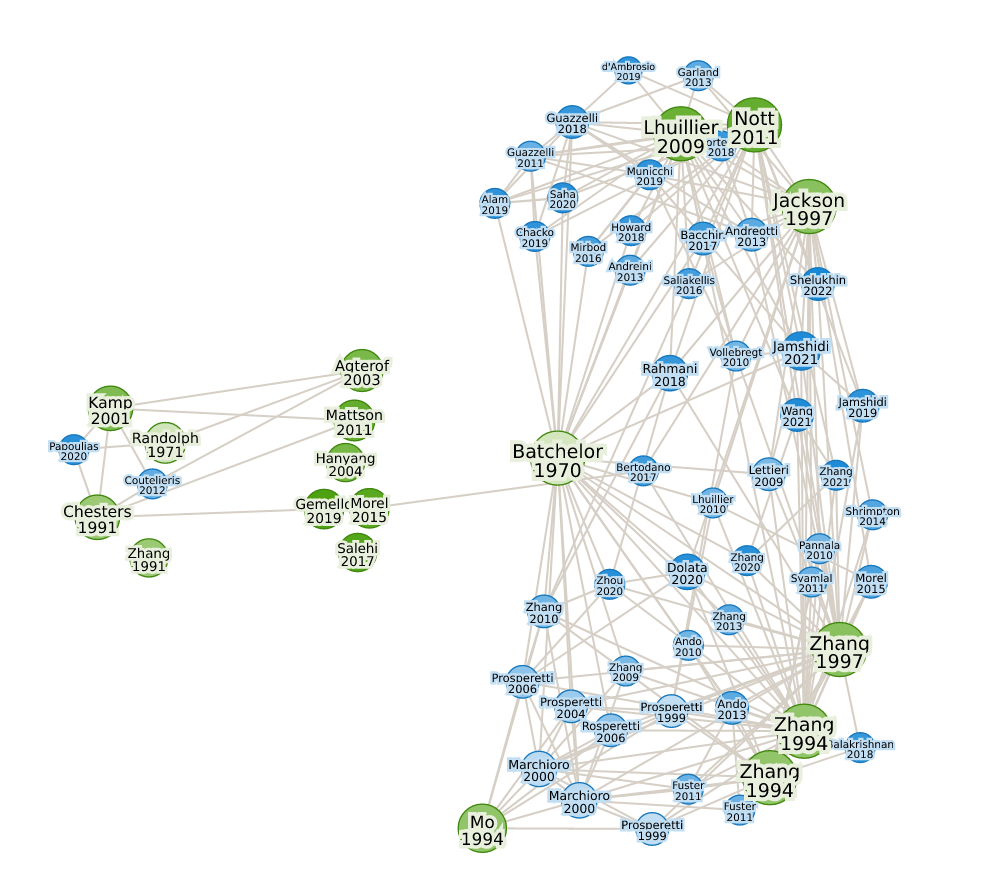
\includegraphics[height=1.8\textheight]{Bib/graph70_paperGraph_network.png}};
\node[thick,text width=6cm](com1) at (-0.35\textwidth,-0.12\textwidth){$\bm{(I)}$Modeling of Coalescence and break up phenomenon, with population balence model (i.e. $S^1$ and $S^2$ transport equtions of \cite{KAMP20011363}) and the closures terms for the frequency Collision and probability of Coalescence \cite{chesters1991modelling} and other\ldots};
\node[thick,text width=6cm](com2) at (0.33\textwidth,-0.15\textwidth){$\bm{(II)}$Ensemble averaging methode for rigide spheres \citep{zhang1994averaged}, and bubbles with variables diameters (no coalescences nor break up) \citep{zhang1997momentum}, the bubbles size are based on Rayleigh–Plesset eq. Closures are proposed in the dillute limite.};
\node[thick,text width=6cm](com3) at (0.33\textwidth,0.17\textwidth){$\bm{(III)}$Local space averaged methode, \cite{jackson1997locally} present closures for spherical solid particles. \cite{Lhuillier_2009},\cite{nott2011suspension} show the importance of the particle phase stress (in $\bm{\Sigma^{(p)}}$) for the migration phenomenon. \cite{batchelor1970stress} made the basis of all theories};
\node[thick,text width=8cm](com1) at (-0.35\textwidth,0.17\textwidth){$\bm{(IV)}$ Population balence model coupled with :  One-way Euler Lagran \citep{mattson2012one},\citep{AGTEROF2003141},  URANS methode \citep{gemello2019population}. Other studies include sphapes of drops \citep{salehi2017population} coupled with probability densities fluctuation of population balance. \citet{morel2015mathematical} gathered ANS and PBM };
\draw[dashed](-1.3,0)ellipse(0.5 and 1.75);
\draw[dashed](-1.3,1.75)node[above]{$\bm{(IV)}$};
\draw[<->](com2.north)--(com3.south)node[midway]{Equivalent};
\end{tikzpicture}
\vfill
\end{frame}
  


\begin{frame}{Closure terms for the population balance equation ($\bm{I}$)}
Model the variation of bubbles population with moment densities \cite{KAMP20011363}. 
  \begin{equation}
    S_\gamma = n\int P(d)d^\gamma\text{d}d
  \end{equation}   
The transport equation for the moments densities $\gamma$ is then :
\begin{equation}
  \frac{\partial S_\gamma}{\partial t}+\nabla\cdot(\bm{u}_\gamma S_\gamma)-\gamma G_{\gamma-1}S_{\gamma-1} = \phi_\gamma
\end{equation}
The closure terms are in the source term $\phi$:
\begin{equation}
  \phi = \int \underbrace{P(d_1,d_2)}_{\text{coalescence probability}}\underbrace{c(d_1,d_2)}_{\text{Collision frequency}}\text{d}d_1\text{d}d_2
\end{equation}
\end{frame}

\begin{frame}
  \frametitle{Navier Stokes Averaged Equations}
\end{frame}

\begin{frame}
  {Volume average method}
  \textbf{Phases fraction and averaging operators : }
  \begin{itemize}
    \item Solid fraction : $\phi(\bm{x},t) = \int g(\bm{x},\bm{y}) \chi(\bm{y},t)dV,$
    \item Fluid fraction : $1 -\phi(\bm{x},t) = \int g(\bm{x},\bm{y}) (1 - \chi(\bm{y},t))dV,$
    \item Number density : $n(\bm{x},t) = \sum_{\alpha} g(\bm{x},\bm{y_\alpha}).$
\end{itemize}

\textit{Fluid-phase average :}
\begin{equation}
  \phi(\bm{x},t)\left<f\right>^d(\bm{x},t) = \int g(\bm{x},\bm{y}) \chi(\bm{y},t) f(\bm{y},t)dV,
  \label{eq:volad}
\end{equation}

\textit{Solid-phase average :}
\begin{equation}
  \label{eq:volaf}
  (1-\phi(\bm{x},t))\left<f\right>^f(\bm{x},t) = \int g(\bm{x},\bm{y}) (1-\chi(\bm{y},t)) f(\bm{y},t)dV,
\end{equation}

\textit{Particles-phase average :}
\begin{equation}
  \label{eq:partia}
  n(\bm{x},t)\left<f\right>^p(\bm{x},t) = \sum_{\alpha} g(\bm{x},\bm{y_\alpha}) f(\bm{y_\alpha},t),
\end{equation}
where $g(\bm{x},\bm{y})$ is the smoothing (or weighting) function.
\end{frame}

\begin{frame}
  {Fluid-phase averaged equations}
  \textbf{Mass conservation :}
  \begin{equation}
    \label{eq:Cmassaf}
    \frac{\partial(1 - \phi)}{\partial t}+\bm{\nabla}\cdot((1-\phi) \left<\bm{u}\right>^f) = 0,
  \end{equation}
  \textbf{Momentum balance :}
  \begin{multline}
    \rho_f\frac{\partial}{\partial t} ((1-\phi)\left<\bm{u}\right>^f) 
    + \rho_f\bm{\nabla}\cdot\left((1-\phi) \left<\bm{u}\right>^f\left<\bm{u}\right>^f\right)
    = (1-\phi)\left<\bm{b}\right>^f 
    +\bm{\nabla}\cdot\left[2 \mu_f\left<\bm{e}\right> -(1-\phi) \left<\bm{p}\right>^f\right]
    \\-n\left<\bm{f}\right>^p
    +\bm{\nabla}\cdot\underbrace{\left[ - \left<\bm{u'u'}\right>^f +n\left<\bm{S^h}\right>^p -\frac{1}{2}\bm{\nabla}(n\left<\bm{Q^h}\right>^p) + \ldots\right]}_{\text{Hydrodynamic particle stress : } \bm{\Sigma^q}},
    \label{eq:favgsp}
\end{multline}
\end{frame}
\begin{frame}
  {Solid-phase and Particles-phase averaged equations}
  \textbf{Mass conservation :}
  \begin{equation}
    \label{eq:Cmassad}
    \frac{\partial \phi}{\partial t}+\bm{\nabla}\cdot(\phi \left<\bm{u}\right>^d) = 0.
\end{equation}
\begin{equation}
  \label{eq:pavgMASS}
  \frac{\partial n}{\partial t} + \bm{\nabla}\left(n\left<\bm{u_\alpha}\right>^p\right) = 0,
\end{equation} 
\textbf{Momentum balance :}
  \begin{equation*}
    \label{eq:davg}
    \rho_d\frac{\partial}{\partial t} (\phi \left<\bm{u}\right>^d) 
    + \rho_d\bm{\nabla}\cdot(\phi \left<\bm{uu}\right>^d)
    = \bm{\nabla}\cdot(\phi \left<\bm{\sigma}\right>^d)
    +\sum_\alpha\int_{S_\alpha}\bm{n}\cdot\bm{\sigma} g dS 
    +\phi\left<\bm{b}\right>^d,
\end{equation*}
\begin{equation}
  \label{eq:pavgsp}
  \rho_d V_\alpha \left[\frac{\partial }{\partial t}(n\left<\bm{u_\alpha}\right>^p) 
  + \bm{\nabla}\cdot(n\left<\bm{u_\alpha}\right>^p\left<\bm{u_\alpha}\right>^p)\right] 
  = n V_\alpha \left<\bm{b}_{ext}\right>^p 
  + n\left<\bm{f_\alpha}\right>^p 
  - \bm{\nabla}\cdot(n\left<\bm{u_\alpha'u_\alpha'}\right>^p),
\end{equation}
\end{frame}
\begin{frame}
  {Angular momentum average :}
  \begin{equation}
    \bm{\mathcal{I}} \left[\frac{\partial}{\partial t}(n\left<\bm{\omega}\right>^p)+\bm{\nabla}\cdot(n\left<\bm{\omega }\right>^p\left<\bm{u_\alpha}\right>^p)\right] = -\bm{\nabla}\cdot(n\left<\bm{\omega'u'}\right>^p) - \bm{\epsilon} : n\left<\bm{S_\alpha}\right>^p + n\left<\bm{\tau_\alpha}\right>^p
    \label{eq:Iavg}
\end{equation}
\end{frame}

\begin{frame}
  \frametitle{How to avoid the expression jump at the interface in the averaged equations.}
  In the dispersed phase average, the 
  

\end{frame}

\begin{frame}{Closure terms in the Volume averaged method considering the fluid phase average and the dispersed phase average}
  Terms related to the \textbf{fluctuations} : 
  \begin{equation}
    \left<u_i'u_k'\right>^f,
    \;\;\left<u_i'u_k'\right>^p,
    \;\;\left<\omega_i'\omega_k'\right>^p,
    \;\;\left<u_i'\omega_k'\right>^p,\;\;
  \end{equation}    
  \begin{itemize}
    \item $\left<\ldots\right>^f$ : Average on the fluid phase (Eulerian phase)
    \item $\left<\ldots\right>^p$ : Average on the particles phase (Lagrangian phase)
  \end{itemize}
  Those quantities are easy to calculate, but the distribution is very sensitive to the size of the domain and mesh refinement.
\end{frame}



\begin{frame}{Closure terms in the Volume averaged method considering the fluid phase average and the dispersed phase average}
  Terms related to \textbf{fluctuations} : 
  \begin{itemize}
    \item $\left<\sigma_{ik}\right>^f = \frac{1}{2}\mu(\nabla\bm{u}+\nabla\bm{u}^T)$ : Averaged stress tensor (Newtonian case).  
    \item $\left<\bm{f}^h\right>^p$ : Averaged hydrodynamic drag forces.  
    \item $\left<\bm{S}^h\right>^p$ : Averaged hydrodynamic 1ft order moment (Stresslet + Torque).  
    \item $\left<\bm{Q}^h\right>^p$ : Averaged hydrodynamic 2nd order moment $\rightarrow$ negligible.  
    \item $\left<\bm{S}^c\right>^p$ : Averaged particular 1ft order moment \citep{nott2011suspension} \citet{zhang2021ensemble} or fluid-particle stress.  
    \item $\left<\bm{Q}^c\right>^p$ : Averaged particular 2nd order moment. $\rightarrow$ negligible.
  \end{itemize}    
\end{frame}

\begin{frame}
  {The hydrodynamic closure terms :}
  
  Force : $$\left<f_i^f\right>^p = \int_S \bm{\sigma\cdot n}dS$$
  
  1st moment : $$\left<\bm{S}^f\right>^p = \sum_\alpha g_\alpha\int_{S_\alpha} (\bm{y} - \bm{y_\alpha})\bm{\sigma\cdot n}dS =  
    + \int_{V_\alpha}\bm{y'}_\alpha \bm{\nabla} \cdot \bm{\sigma} dV- \int_{V_\alpha} \bm{\sigma} dV$$
  

  $\rightarrow$ How to calculate the hydrodynamic 1ft order moment on basilisk ?
  
  2nd moment : $$\left<\bm{Q}^f\right>^p = \sum_i g_i\int_{S_i} (\bm{x} - \bm{x_i})(\bm{x} - \bm{x_i})\bm{\sigma\cdot n}dS \approx 0$$

  where $x_i$, $S_i$ and $g_i$ are respectively, the center, the surface and the weight function value at the $i$ particle. 


\end{frame}
\begin{frame}
  {The particular stress closure terms :}

  1st moment : $$\left<\bm{S}^c\right>^p = \bm{\Sigma}_{FPF}$$

  This can be found either in \citet{nott2011suspension} for Stokesian suspensions or in \citet{zhang2021ensemble} and \citet{wang2021numerical} for a more general case.
\end{frame}


\begin{frame}
  \frametitle{Closure for the averaged force :}
  \begin{figure}[h!]
    \centering
    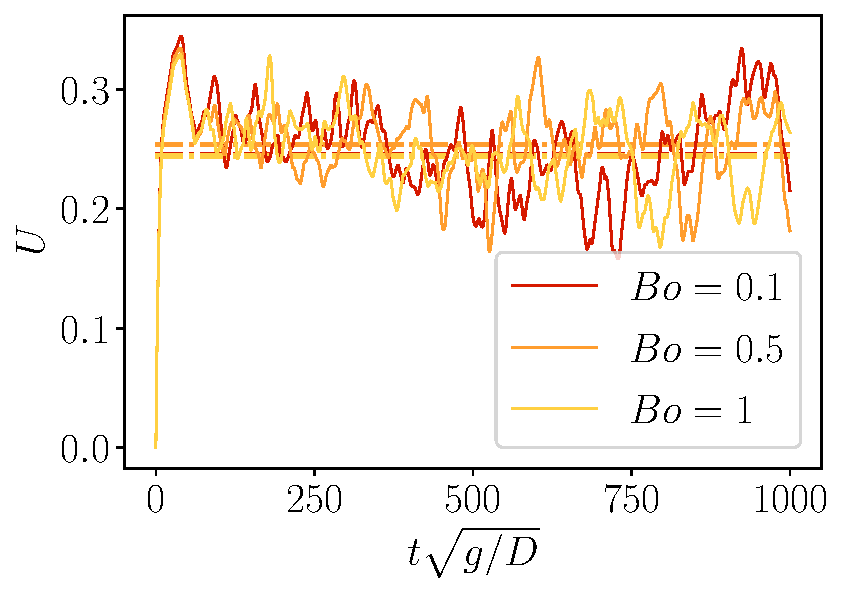
\includegraphics[height=0.5\textheight]{image/N_10/Favg/Bosdep_Ga_50.pdf}
    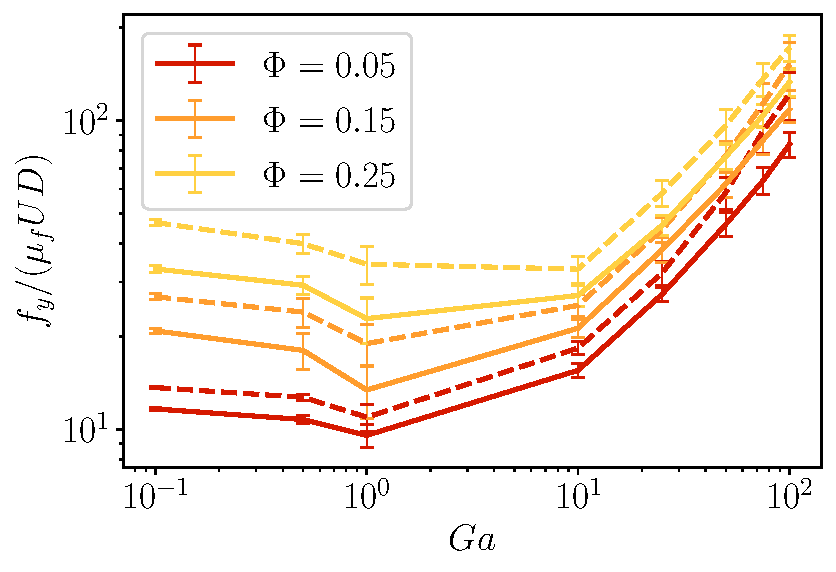
\includegraphics[height=0.5\textheight]{image/N_10/Favg/F_mu_Bo_0_5.pdf}
    \caption{(left) : Relative velocity in terms of the dimensionless time for different $Bo$ for $\phi = 0.15$, $\mu_r = 0.042$ and $Ga = 50$. (right) : Averaged drag force per droplets. Dashed lines : $\mu_f = 0.42$, solid lines : $\mu_f = 0.042$. The results are shown for $Bo = 0.5$.} 
    \label{fig:avgF}
\end{figure}
$\rightarrow$ No variation when $Bo\in[0;1]$
\end{frame}
\begin{frame}
  \frametitle{Closure for the fluid averaged pseudo turbulent tensor }
  \begin{figure}[h!]
    \centering
    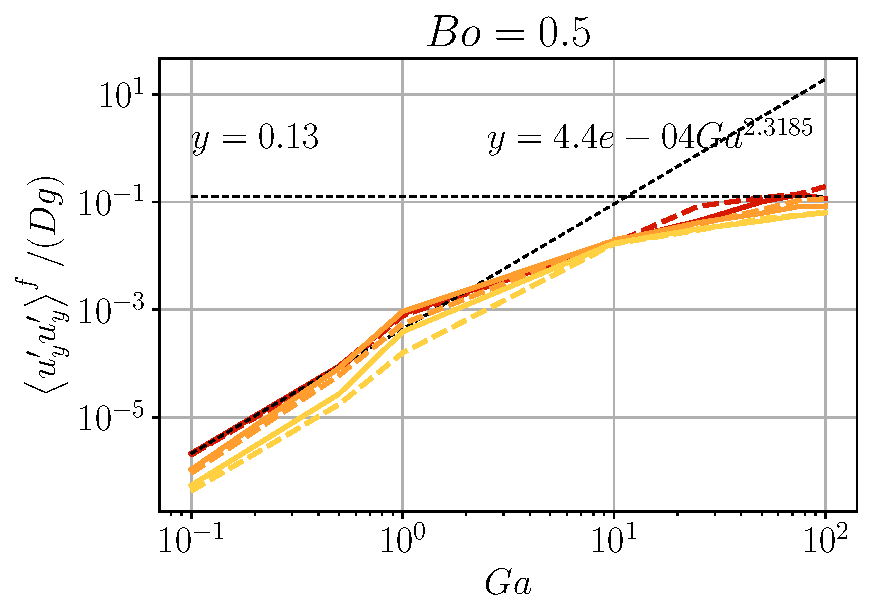
\includegraphics[height=0.5\textheight]{image/N_10/UU/UU_fyy_Bo_0_5.pdf}
    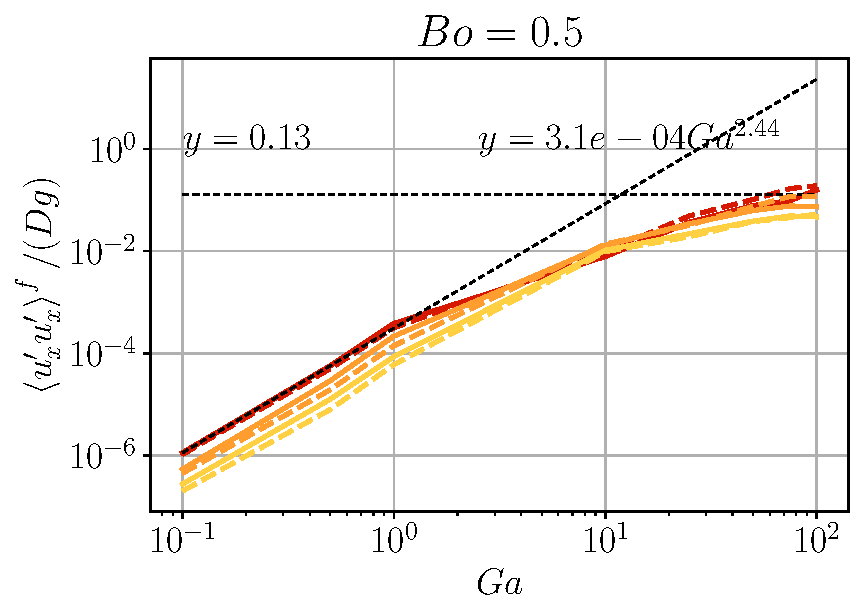
\includegraphics[height=0.5\textheight]{image/N_10/UU/UU_fxx_Bo_0_5.pdf}
    \caption{Fluid-phase average of the dimensionless velocity fluctuations. Dashed lines : $\mu_f = 0.42$, solid lines : $\mu_f = 0.042$, Dotted lines : asymptotic fit for $\phi = 0.05$ and $\mu_r = 0.42$. The results are shown for $Bo = 0.5$.} 
    \label{fig:UUf}
  \end{figure} 
  $\rightarrow$ No variation when $Bo\in[0;1]$
\end{frame}

\begin{frame}
  \frametitle{Closure for the particles phase average pseudo turbulent tensor : }
  \begin{figure}[h!]
    \centering
    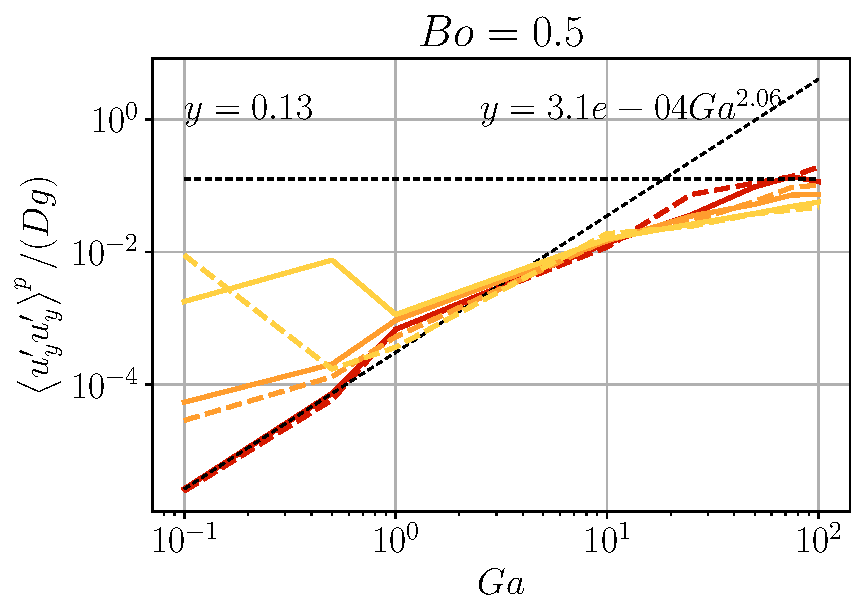
\includegraphics[height=0.5\textheight]{image/N_10/UU/UU_pyy_Bo_0_5.pdf}
    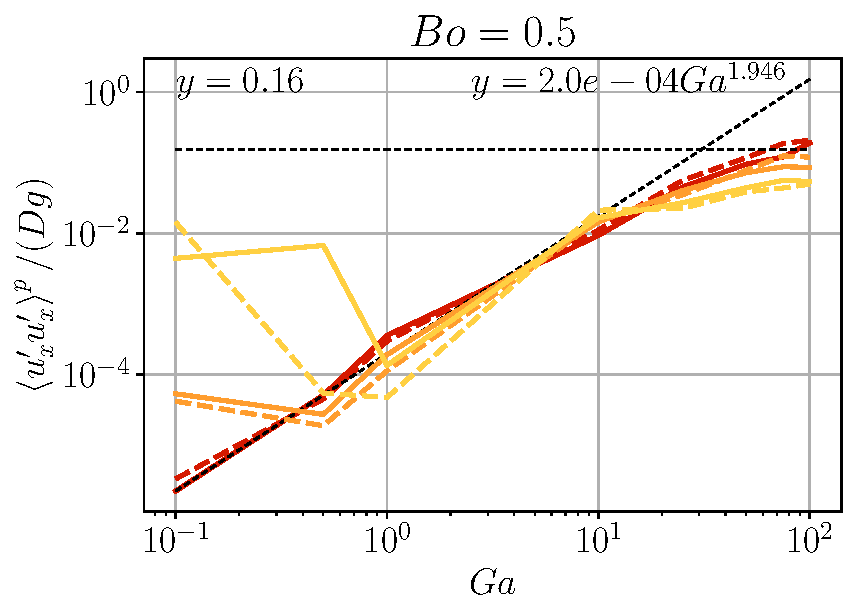
\includegraphics[height=0.5\textheight]{image/N_10/UU/UU_pxx_Bo_0_5.pdf}
    \caption{Fluid-phase average of the dimensionless velocity fluctuations. Dashed lines : $\mu_f = 0.42$, solid lines : $\mu_f = 0.042$, Dotted lines : asymptotic fit for $\phi = 0.05$ and $\mu_r = 0.42$. The results are shown for $Bo = 0.5$.} 
    \label{fig:UUp}
  \end{figure}
  

\end{frame}
\section*{Averaged equation for a poly-dispersed suspension of fluid particles}
\begin{frame}
  \vfill
  \centering
  \Huge{Averaged equation for a poly-dispersed suspension of fluid particles}
  \vfill
\end{frame}
\begin{frame}
  \frametitle{Newton second law of motion for fluid particles.}
  The mass, $m_\alpha$, the momentum $\bm{p}_\alpha$ and \textit{moment of momentum} $\bm{P}_\alpha$ of a deformable particle $\alpha$, are defined such that,
  \begin{equation}
      m_\alpha = \int_{V_\alpha} \rho_d dV,\;\;\;
      \bm{p}_\alpha = \int_{V_\alpha} \rho_d \bm{u} dV,\;\;\;
      \bm{P}_\alpha = \int_{V_\alpha} \rho_d \bm{u}\\bm{r}_\alpha dV,
  \end{equation}
  where $V_\alpha$ is the volume of the particle $\alpha$.
  $\\bm{r}_\alpha$ is defined such that, $\\bm{r}_\alpha = \bm{y} - \bm{y_\alpha}$ with $m_\alpha\bm{y_\alpha} = \int_{V_\alpha} \rho_d\bm{y}dV$ is still the center of mass of the particle $\alpha$. 
  We note $\bm{u}_\alpha = d\bm{y}_\alpha/dt$ the velocity of the center of mass $\alpha$, and we define the fluctuation velocity around $\bm{u}_\alpha$ as $\bm{u''}_\alpha = \bm{u} - \bm{u}_\alpha$.
  Then we can rewrite the above set of equations as, 
  \begin{equation}
      \bm{p}_\alpha = m_\alpha \bm{u}_\alpha 
      + \int_{V_\alpha} \rho_d \bm{u''}_\alpha dV,\;\;\;
      \bm{P}_\alpha = \int_{V_\alpha} \rho_d \bm{u''}_\alpha\\bm{r}_\alpha dV.
  \end{equation}
\end{frame}
\begin{frame}
  \frametitle{Newton second law of motion for fluid particles.}
  Using Navier stokes equation and Reynolds transport theorem, it yields,
  \begin{equation}
    \frac{d m_\alpha}{dt} 
    = \underbrace{\int_{S_\alpha} T_\alpha dS}_{\text{Mass transfer}},
  \end{equation}    
  \begin{equation}
    \frac{d\bm{p}_\alpha}{dt} 
    = \int_{V_\alpha} \bm{u} \rho_d dV 
    = \underbrace{\int_{V_\alpha} \bm{b} dV}_{\text{Body forces}} 
    + \underbrace{\int_{S_\alpha} \bm{\sigma}_f \cdot \bm{n} dS}_{\text{External forces}}
    + \underbrace{\int_{S_\alpha} \bm{u} T_\alpha dS}_{\text{Momentum mass transfer}}
  \end{equation}
\end{frame}
\begin{frame}
  \frametitle{Newton second law of motion for fluid particles.}
We can rewrite the momentum balance as such,
\begin{equation}
  \frac{d m_\alpha \bm{u}_{\alpha}}{dt} 
  = V_\alpha\bm{b}^{\text{ext}} 
  + \bm{f}_\alpha
  + \int_{S_\alpha} \bm{u} T_\alpha dS
  - \frac{d}{dt}  \int_{V_\alpha} \rho_d \bm{u''}_\alpha dV.
\end{equation}
From now on we neglect the mass transfer, 
\begin{equation}
  \label{eq:massdef}
  \frac{d m_\alpha}{dt} 
  = 0,
\end{equation}
\begin{equation}
  \label{eq:momentumdef}
  \frac{d \bm{p_\alpha}}{dt} 
  = \rho_d \frac{d}{dt} \left(V_\alpha \bm{u_\alpha} 
  + \int_{V_\alpha} \bm{u''}_\alpha dV\right)
  = V_\alpha\bm{b}_{\text{ext}} 
  + \bm{f}_\alpha,
\end{equation}
\end{frame}
\begin{frame}
  \frametitle{Particles Mass averaged equation}
  \begin{equation}
    \frac{\partial }{\partial t}(n\left<V_\alpha\right>^p) 
    + \bm{\nabla}\cdot(n\left<V_\alpha\right>^p\left<\bm{u_\alpha}\right>^p )
    = 
    - \bm{\nabla}\cdot(n\left<\bm{u'_\alpha}V'_\alpha\right>^p),
\end{equation}  
where, $V_\alpha'$ is the fluctuations around the mean value of $V_\alpha$,
namely, $V_\alpha' = V_\alpha - \left<V_\alpha\right>$.
Since $nV_\alpha = \phi$,
\begin{equation}
  \frac{\partial }{\partial t}(\phi) 
  + \bm{\nabla}\cdot(\phi\left<\bm{u_\alpha}\right>^p )
  = 
  - \bm{\nabla}\cdot(n\left<\bm{u'_\alpha}V'_\alpha\right>^p).
  \label{eq:massavg}
\end{equation}  
If we consider, $\left<\bm{u_\alpha}\right>^p =\left<\bm{u_\alpha}\right>^d + \mathcal{O}\left(L/l\right)$,
with $L$ the size of the particles and $l$ the radius of $g$. 

Then, by identification with the dispersed-phase average mass balance equation it yields,
\begin{equation}
  - \bm{\nabla}\cdot(n\left<\bm{u'_\alpha}V'_\alpha\right>^p) =  \mathcal{O}\left(L/l\right)
\end{equation}
\end{frame}
\begin{frame}
  \frametitle{Momentum balance equation}
  \begin{multline}
    \rho_d 
    \frac{\partial }{\partial t}
    \left[
        \phi \left<\bm{u}_\alpha\right>^p
    \right] 
    + \rho_d\bm{\nabla}\cdot
    \left[
        \phi \left<\bm{u}_\alpha\right>^p \left<\bm{u}_\alpha\right>^p
    + \left<\bm{u_\alpha}\right>^p \bm{F_1}
    \right]
    \\= n \left<V_\alpha\right>^p\bm{b_{ext}} 
    + n\left<\bm{f_\alpha}\right>^p
    - \frac{\partial }{\partial t}\bm{F_2},
    - \bm{\nabla}\cdot\bm{F_3},
    \label{eq:particlesAVG}
\end{multline} 
where,
\begin{equation*}
    \bm{F_1}
    = 2\left<V_\alpha'\bm{u}_\alpha'\right>^p
    +  \left<\int_{V_\alpha} \bm{u''_\alpha}dV\right>^p,
\end{equation*} 
\begin{equation*}
    \bm{F_2}/\rho_d
    = \left<\int_{V_\alpha} \bm{u''_\alpha}dV\right>^p,
\end{equation*}
and
\begin{equation*}
    \bm{F_3}/\rho_d
    = \left<V_\alpha' \bm{u}_\alpha'\bm{u}_\alpha'\right>^p
    + \left<V_\alpha\right>^p \left<\bm{u}_\alpha'\bm{u}_\alpha'\right>^p
    +\left<\bm{u_\alpha}'\left(\int_{V_\alpha} \bm{u''_\alpha}dV\right)'\right>^p.
\end{equation*}
  

\end{frame}




















\section*{Conditional property}
\begin{frame}
  \vfill
  \centering
  \Huge{Conditional property}
  \vfill
\end{frame}
\begin{frame}{Set of data :}

  \begin{itemize}
    \item Bi periodic simulations of $N_b = 100$ drops for $1000$ second. 
    \item  The Galileo number $Ga = 10 \rightarrow 100$. 
    \item  The drops volume fraction $\phi = 0.15 \rightarrow 0.35$ 
    \item  And the viscosity ratio from $\mu_r = \mu_f/\mu_d = 0.042 \rightarrow 0.35$ 
    \item  We keep the Eötvös or Bond number $Bo = 0.5$.  
  \end{itemize}
\end{frame}

\begin{frame}
  {Definition}
  We wish to evaluate a quantity $q$ of a particle, being at the position $\bm{x}$, knowing that the nearest particle is at the position $\bm{y}$. 
  Then we average by range of $r = |\bm{x} - \bm{y}|$, on all the possible configuration of the flow (time space and time). 

  Following this method, we can evaluate any quantity $q$, or relative quantity $q_{rel}$ knowing that the distance with the closed neighboring particle is $r$.

  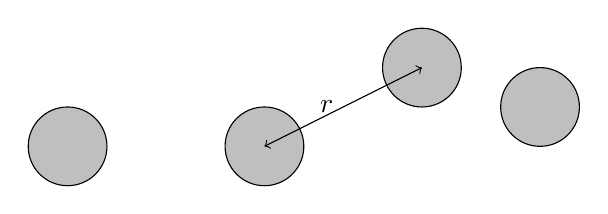
\begin{tikzpicture}
    \draw[fill=gray!50] (0,0)circle(0.5);
    \draw[fill=gray!50] (2,1)circle(0.5);
    \draw[fill=gray!50] (3.5,0.5)circle(0.5);
    \draw[fill=gray!50] (-2.5,0)circle(0.5);
    \draw[<->](0,0)--(2,1)node[midway,left]{$r$};
  \end{tikzpicture}
\end{frame}
\begin{frame}
  {Probably density function :}
  \begin{figure}
    \centering
    \includegraphics[height=  0.25\textwidth]{image/N_10/Pcond/Distrib0_15mu_0_42.pdf}
    \includegraphics[height=  0.25\textwidth]{image/N_10/Pcond/Distrib0_35mu_0_42.pdf}
  \end{figure}
  \begin{itemize}
  \item The maximum distance $r_{max}$, at which the density isn't null, is the average distance between particles in a homogeneous suspension. There for in average $r_max  = \sqrt{\frac{\pi D^2}{4 \phi}}$ 
\end{itemize} 
\end{frame}
\begin{frame}
  {Probably density function :}
  \begin{figure}
    \centering
    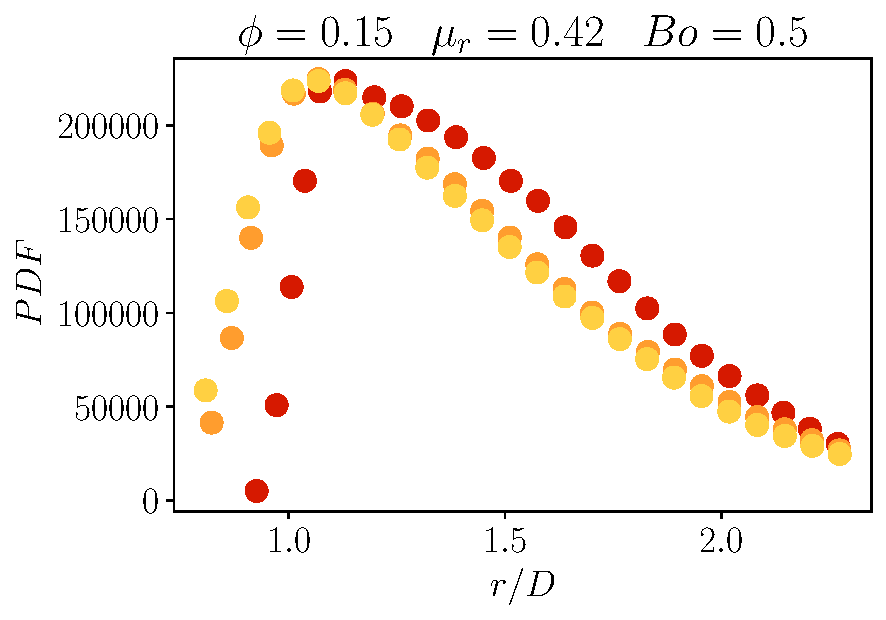
\includegraphics[height=  0.25\textwidth]{image/N_10/Pcond/Distrib0_15mu_0_42Bo_0_5.pdf}
    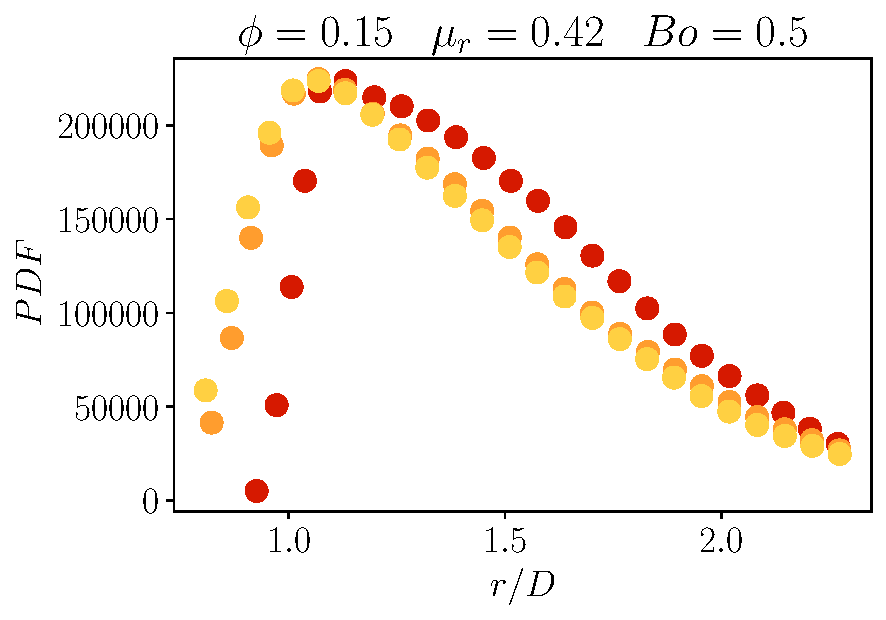
\includegraphics[height=  0.25\textwidth]{image/N_10/Pcond/Distrib0_15mu_0_42Bo_0_5.pdf}
  \end{figure}
  \begin{itemize}
    \item The nearest neighboring particle density is closer with growing $Ga$ since inertial effect are more susceptible to deform particles, thus they end up closer. 
  \end{itemize} 
\end{frame}

\begin{frame}
  {Relative velocity $v_{rel}$}
  \begin{figure}
    \centering
    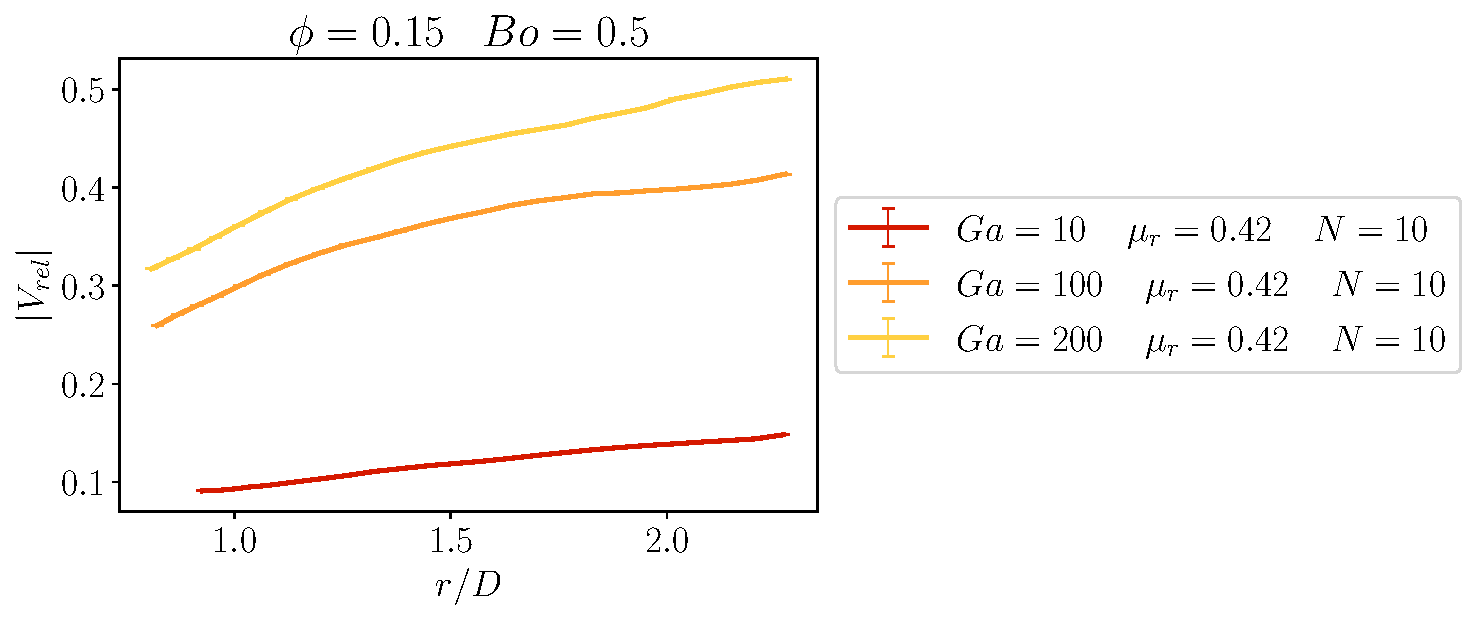
\includegraphics[height=  0.25\textwidth]{image/N_10/Pcond/probav_rel0_15Bo_0_5.pdf}
  \end{figure}
  \begin{itemize}
    \item The velocity decrease with smaller $r$. 
    \item The maximum velocity is higher for dilute suspensions (because the distance $r_max$ is bigger). 
    \item Can be usefull for $\lambda$ . 
  \end{itemize} 
\end{frame}
\begin{frame}
  {Relative acceleration $a_{rel}$}
  \begin{figure}
    \centering
    \includegraphics[height=  0.25\textwidth]{image/N_10/Pcond/probaa_rel0_15.pdf}
    \includegraphics[height=  0.25\textwidth]{image/N_10/Pcond/probaa_rel0_35.pdf}
  \end{figure}
  \begin{itemize}
    \item The acceleration is rather constant until $r<1$
  \end{itemize}
\end{frame}
\begin{frame}
  {Relative rotational velocity $\Omega_{rel}$}
  \begin{figure}
    \centering
    \includegraphics[height=  0.25\textwidth]{image/N_10/Pcond/probaomegaz_rel0_15.pdf}
    \includegraphics[height=  0.25\textwidth]{image/N_10/Pcond/probaomegaz_rel0_35.pdf}
  \end{figure}
  \begin{itemize}
    \item The rotational velocity of two bubble decrease with the contact, thus they roll on each other.
    \item For high $\phi$ it is less obvious. 
  \end{itemize}
\end{frame}
\begin{frame}
  {Viscous dissipation $|\bm{\tau}| = 0.5\left(\nabla \bm{u}+\nabla \bm{u}^T\right)$}
  \begin{figure}
    \centering
    \includegraphics[height=  0.25\textwidth]{image/N_10/Pcond/probadiss0_15.pdf}
    \includegraphics[height=  0.25\textwidth]{image/N_10/Pcond/probadiss0_35.pdf}
  \end{figure}
\end{frame}
\begin{frame}
  {Relative kinetic energy  $E_c = 1/2 m |\bm{v}{rel}|^2$}
  \begin{figure}
    \centering
    \includegraphics[height=  0.25\textwidth]{image/N_10/Pcond/probaE_crel0_15.pdf}
    \includegraphics[height=  0.25\textwidth]{image/N_10/Pcond/probaE_crel0_35.pdf}
  \end{figure}
\end{frame}

\begin{frame}
  {Norm of the deformation  $\bm{\sigma}$}
  \begin{figure}
    \centering
    \includegraphics[height=  0.25\textwidth]{image/N_10/Pcond/probadefnorm0_15.pdf}
    \includegraphics[height=  0.25\textwidth]{image/N_10/Pcond/probadefnorm0_35.pdf}
  \end{figure}
  \begin{itemize}
    \item calculation of the surface energy instead. 
    \item $(E_c + E_\Omega )+E_\sigma +\tau = constant$
  \end{itemize}
\end{frame}

\begin{frame}
   {High standard deviation}

\end{frame}

\begin{frame}
  {Collision oriention}
  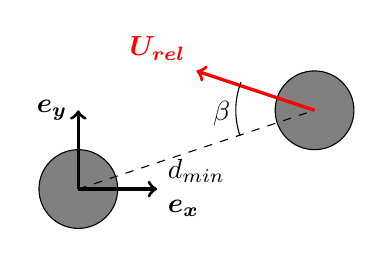
\begin{tikzpicture}
    \draw[fill=gray](0,0)circle (0.5);
    \draw[fill=gray](3,1)circle (0.5);
    \draw[dashed](0,0)--(3,1)node[midway,below]{$d_{min}$};
    \draw[very thick,->,red](3,1)--++(-1.5,0.5)node[above left]{$\bm{U_{rel}}$};
    \draw[very thick,->](0,0)--++(1,0)node[below right]{$\bm{e_x}$};
    \draw[very thick,->](0,0)--++(0,1)node[left]{$\bm{e_y}$};
    \draw(3,1)++(199:1)node[above left]{$\beta$} arc(199:159:1);
  \end{tikzpicture} 
  \begin{figure}
    \includegraphics[width=1.2\textheight]{image/N_10/beta/Vrel_PbVsb.pdf}
  \end{figure}
\end{frame}

\begin{frame}
  {Collision oriention}
  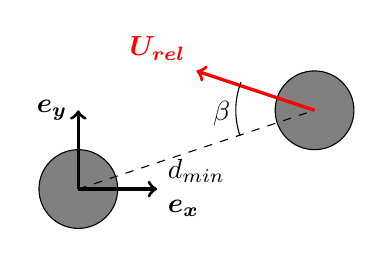
\begin{tikzpicture}
    \draw[fill=gray](0,0)circle (0.5);
    \draw[fill=gray](3,1)circle (0.5);
    \draw[dashed](0,0)--(3,1)node[midway,below]{$d_{min}$};
    \draw[very thick,->,red](3,1)--++(-1.5,0.5)node[above left]{$\bm{U_{rel}}$};
    \draw[very thick,->](0,0)--++(1,0)node[below right]{$\bm{e_x}$};
    \draw[very thick,->](0,0)--++(0,1)node[left]{$\bm{e_y}$};
    \draw(3,1)++(199:1)node[above left]{$\beta$} arc(199:159:1);
  \end{tikzpicture} 
  \begin{figure}
    \includegraphics[width=1.2\textheight]{image/N_10/beta/Vrel_PbSdminVsb.pdf}
  \end{figure}
\end{frame}
\begin{frame}
  {Collision oriention}
  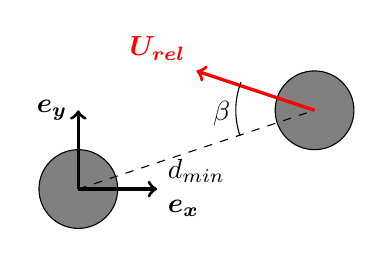
\begin{tikzpicture}
    \draw[fill=gray](0,0)circle (0.5);
    \draw[fill=gray](3,1)circle (0.5);
    \draw[dashed](0,0)--(3,1)node[midway,below]{$d_{min}$};
    \draw[very thick,->,red](3,1)--++(-1.5,0.5)node[above left]{$\bm{U_{rel}}$};
    \draw[very thick,->](0,0)--++(1,0)node[below right]{$\bm{e_x}$};
    \draw[very thick,->](0,0)--++(0,1)node[left]{$\bm{e_y}$};
    \draw(3,1)++(199:1)node[above left]{$\beta$} arc(199:159:1);
  \end{tikzpicture} 
  \begin{figure}
    \includegraphics[width=1.2\textheight]{image/N_10/beta/Arel_PbVsb.pdf}
  \end{figure}
\end{frame}
\begin{frame}
  {Collision oriention}
  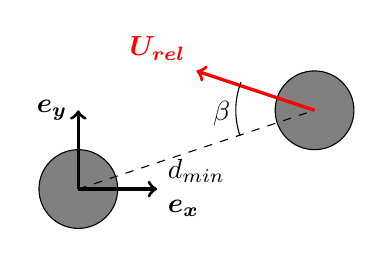
\begin{tikzpicture}
    \draw[fill=gray](0,0)circle (0.5);
    \draw[fill=gray](3,1)circle (0.5);
    \draw[dashed](0,0)--(3,1)node[midway,below]{$d_{min}$};
    \draw[very thick,->,red](3,1)--++(-1.5,0.5)node[above left]{$\bm{U_{rel}}$};
    \draw[very thick,->](0,0)--++(1,0)node[below right]{$\bm{e_x}$};
    \draw[very thick,->](0,0)--++(0,1)node[left]{$\bm{e_y}$};
    \draw(3,1)++(199:1)node[above left]{$\beta$} arc(199:159:1);
  \end{tikzpicture} 
  \begin{figure}
    \includegraphics[width=1.2\textheight]{image/N_10/beta/Arel_PbSdminVsb.pdf}
  \end{figure}
\end{frame}



\bibliography{Bib/bib_bulles.bib}

\end{document}

